    \documentclass[11pt]{article}

    \usepackage[a4paper,top=2.0cm,bottom=2.2cm,left=2.0cm,right=2.0cm]{geometry}
    \usepackage[utf8]{inputenc}
    \usepackage[T1]{fontenc}
    \usepackage{times}
    \usepackage{microtype}
    \usepackage{xcolor}
    \usepackage{graphicx}
    \usepackage{booktabs}
    \usepackage{array}
    \usepackage{tabularx}
    \usepackage{amsmath,amssymb}
    \usepackage{caption}
    \usepackage{float}
    \usepackage{placeins}
    \usepackage{algorithm}
    \usepackage{algorithmic}
    \usepackage{xurl}
    \usepackage[colorlinks=true,linkcolor=blue,citecolor=blue,urlcolor=blue]{hyperref}
    \hypersetup{
      pdftitle={Supplementary Information for SoftFuse-KGC: Soft Support and Confidence-Aware Fuzzy Retrieval for Biomedical Knowledge Graph Completion},
      pdfauthor={Dang Hoang Duong, Le Van Thanh, Hai Van Pham},
      pdfsubject={Online Resource 1 for Network Modeling Analysis in Health Informatics and Bioinformatics},
      pdfkeywords={Biomedical knowledge graph; Knowledge graph completion; Drug repurposing; Soft evidence modeling; Fuzzy retrieval}
    }

    \newcommand{\softfuse}{SoftFuse-KGC}
    \newcommand{\drkgc}{DrKGC}
    \newcommand{\mainsec}[1]{Section~#1}
    \newcommand{\mainequation}[1]{Eq.~(#1)}
    \newcommand{\mrr}{MRR@20}
    \newcommand{\gold}{Gold@20}
    \newcommand{\hitsten}{Hits@10}
    \newcolumntype{Y}{>{\raggedright\arraybackslash}X}
    \newcolumntype{L}[1]{>{\raggedright\arraybackslash}p{#1}}

    \renewcommand{\thetable}{S\arabic{table}}
    \renewcommand{\thefigure}{S\arabic{figure}}
    \renewcommand{\thealgorithm}{S\arabic{algorithm}}
    \renewcommand{\thesection}{S\arabic{section}}
    \renewcommand{\thesubsection}{S\arabic{section}.\arabic{subsection}}
    \renewcommand{\arraystretch}{1.15}
    \setlength{\parindent}{0pt}
    \setlength{\parskip}{0.45em}
    \captionsetup{font=small,labelfont=bf,labelsep=space}
    \captionsetup[figure]{name=Fig.}

    \begin{document}
    \begin{center}
    {\Large\bfseries Supplementary Materal\par}
    \vspace{0.8em}
%    {\large\bfseries SoftFuse-KGC: Soft Support and Confidence-Aware Fuzzy Retrieval for Biomedical Knowledge Graph Completion\par}
%    \vspace{0.8em}
%    {\itshape Network Modeling Analysis in Health Informatics and Bioinformatics\par}
%    \vspace{0.9em}
%    Dang Hoang Duong\(^{1,\dagger}\), Le Van Thanh\(^{2,3,\dagger}\), and Hai Van Pham\(^{1,*}\)\par
%    \vspace{0.5em}
%    {\small
%    \(^{1}\)School of Information and Communications Technology, Hanoi University of Science and Technology, Hanoi, Vietnam\par
%    \(^{2}\)Cyber School, Vinh University, Vinh, Nghe An, Vietnam\par
%    \(^{3}\)Graduate University of Science and Technology, Vietnam Academy of Science and Technology, Hanoi, Vietnam\par}
    \end{center}

%	\(^{\dagger}\)These authors contributed equally to this work.
%
%    \noindent\textbf{Corresponding author}\par
%    \noindent Hai Van Pham, School of Information and Communications Technology, Hanoi University of Science and Technology, Hanoi, Vietnam; email: \href{mailto:haipv@soict.hust.edu.vn}{haipv@soict.hust.edu.vn}
%
%    \medskip
%    \noindent\textbf{Online Resource 1}\par
%    \noindent\textbf{File:} ESM\_1.pdf\par
%    \noindent\textbf{Caption:} Supplementary methods, implementation details, web-application instructions, validation analyses, robustness checks, and dataset preprocessing information for SoftFuse-KGC

    \medskip
    \hrule
    \bigskip

    \section*{The Web Application}

    We provide a public web application for interactive inspection of the \softfuse{} pipeline at:
    \url{https://inosuke710-softfuse-kgc-demo.hf.space/}. The web application is a demonstration deployed on Hugging Face Spaces and uses precomputed artifacts. It allows users to inspect validation and test examples across PrimeKG, PharmKG, Hetionet, DRKG, and repoDB. After opening the page, users select a dataset, split, disease/query case, and top-\(k\) value. The three main tabs then expose the complete demo flow: an overall prediction summary, candidate reranking by soft support, and evidence-subgraph selection by fuzzy retrieval.

    Figures~\ref{fig:s1_overview}--\ref{fig:s3_fuzzy_retrieval} document the three tabs and identify the controls, result panels, candidate lists, graph elements, and visual encodings used in the interface.

    \begin{figure}[H]
    \centering
    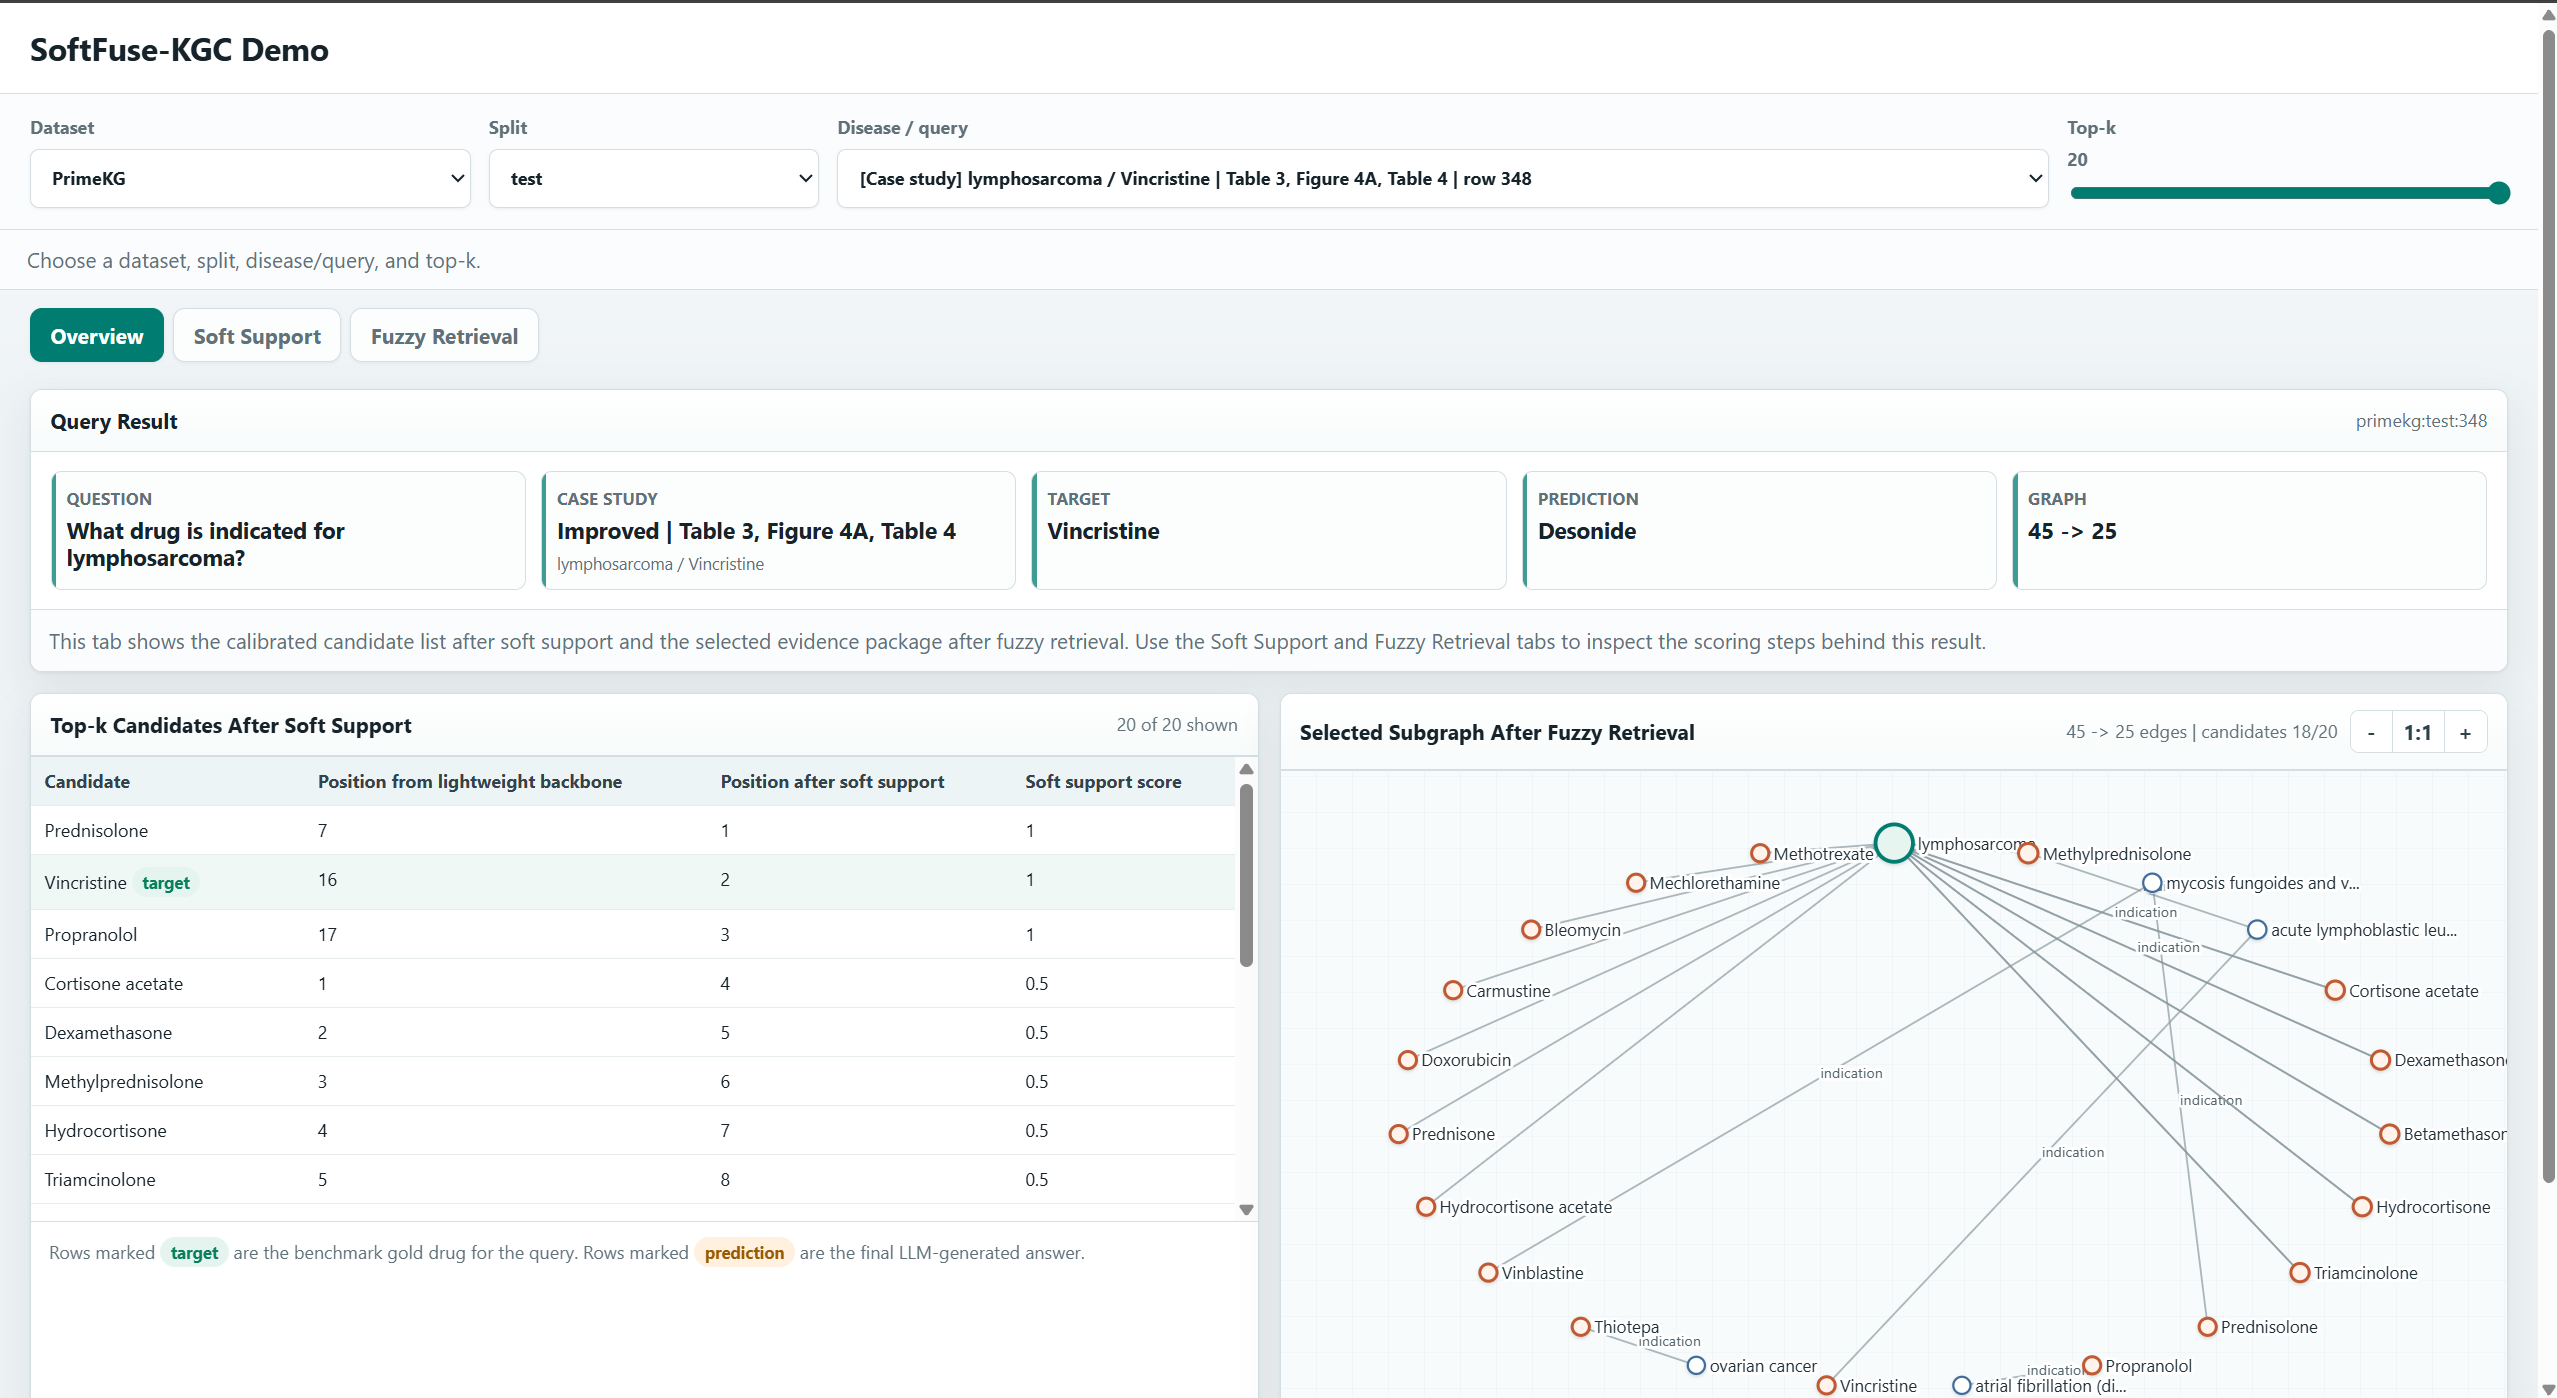
\includegraphics[width=\textwidth]{FigS1.png}
    \caption{\textbf{Overview tab.} Controls select the dataset, evaluation split, disease or query case, and displayed top-\(k\). The Query Result panel reports the question, case-study label when available, gold target, prediction, and graph-compression size. The candidate table gives backbone rank, calibrated rank, and soft-support score, with text markers for the target and prediction. The graph panel shows the selected fuzzy evidence subgraph and provides zoom, reset, and drag controls}
    \label{fig:s1_overview}
    \end{figure}

    \begin{figure}[H]
    \centering
    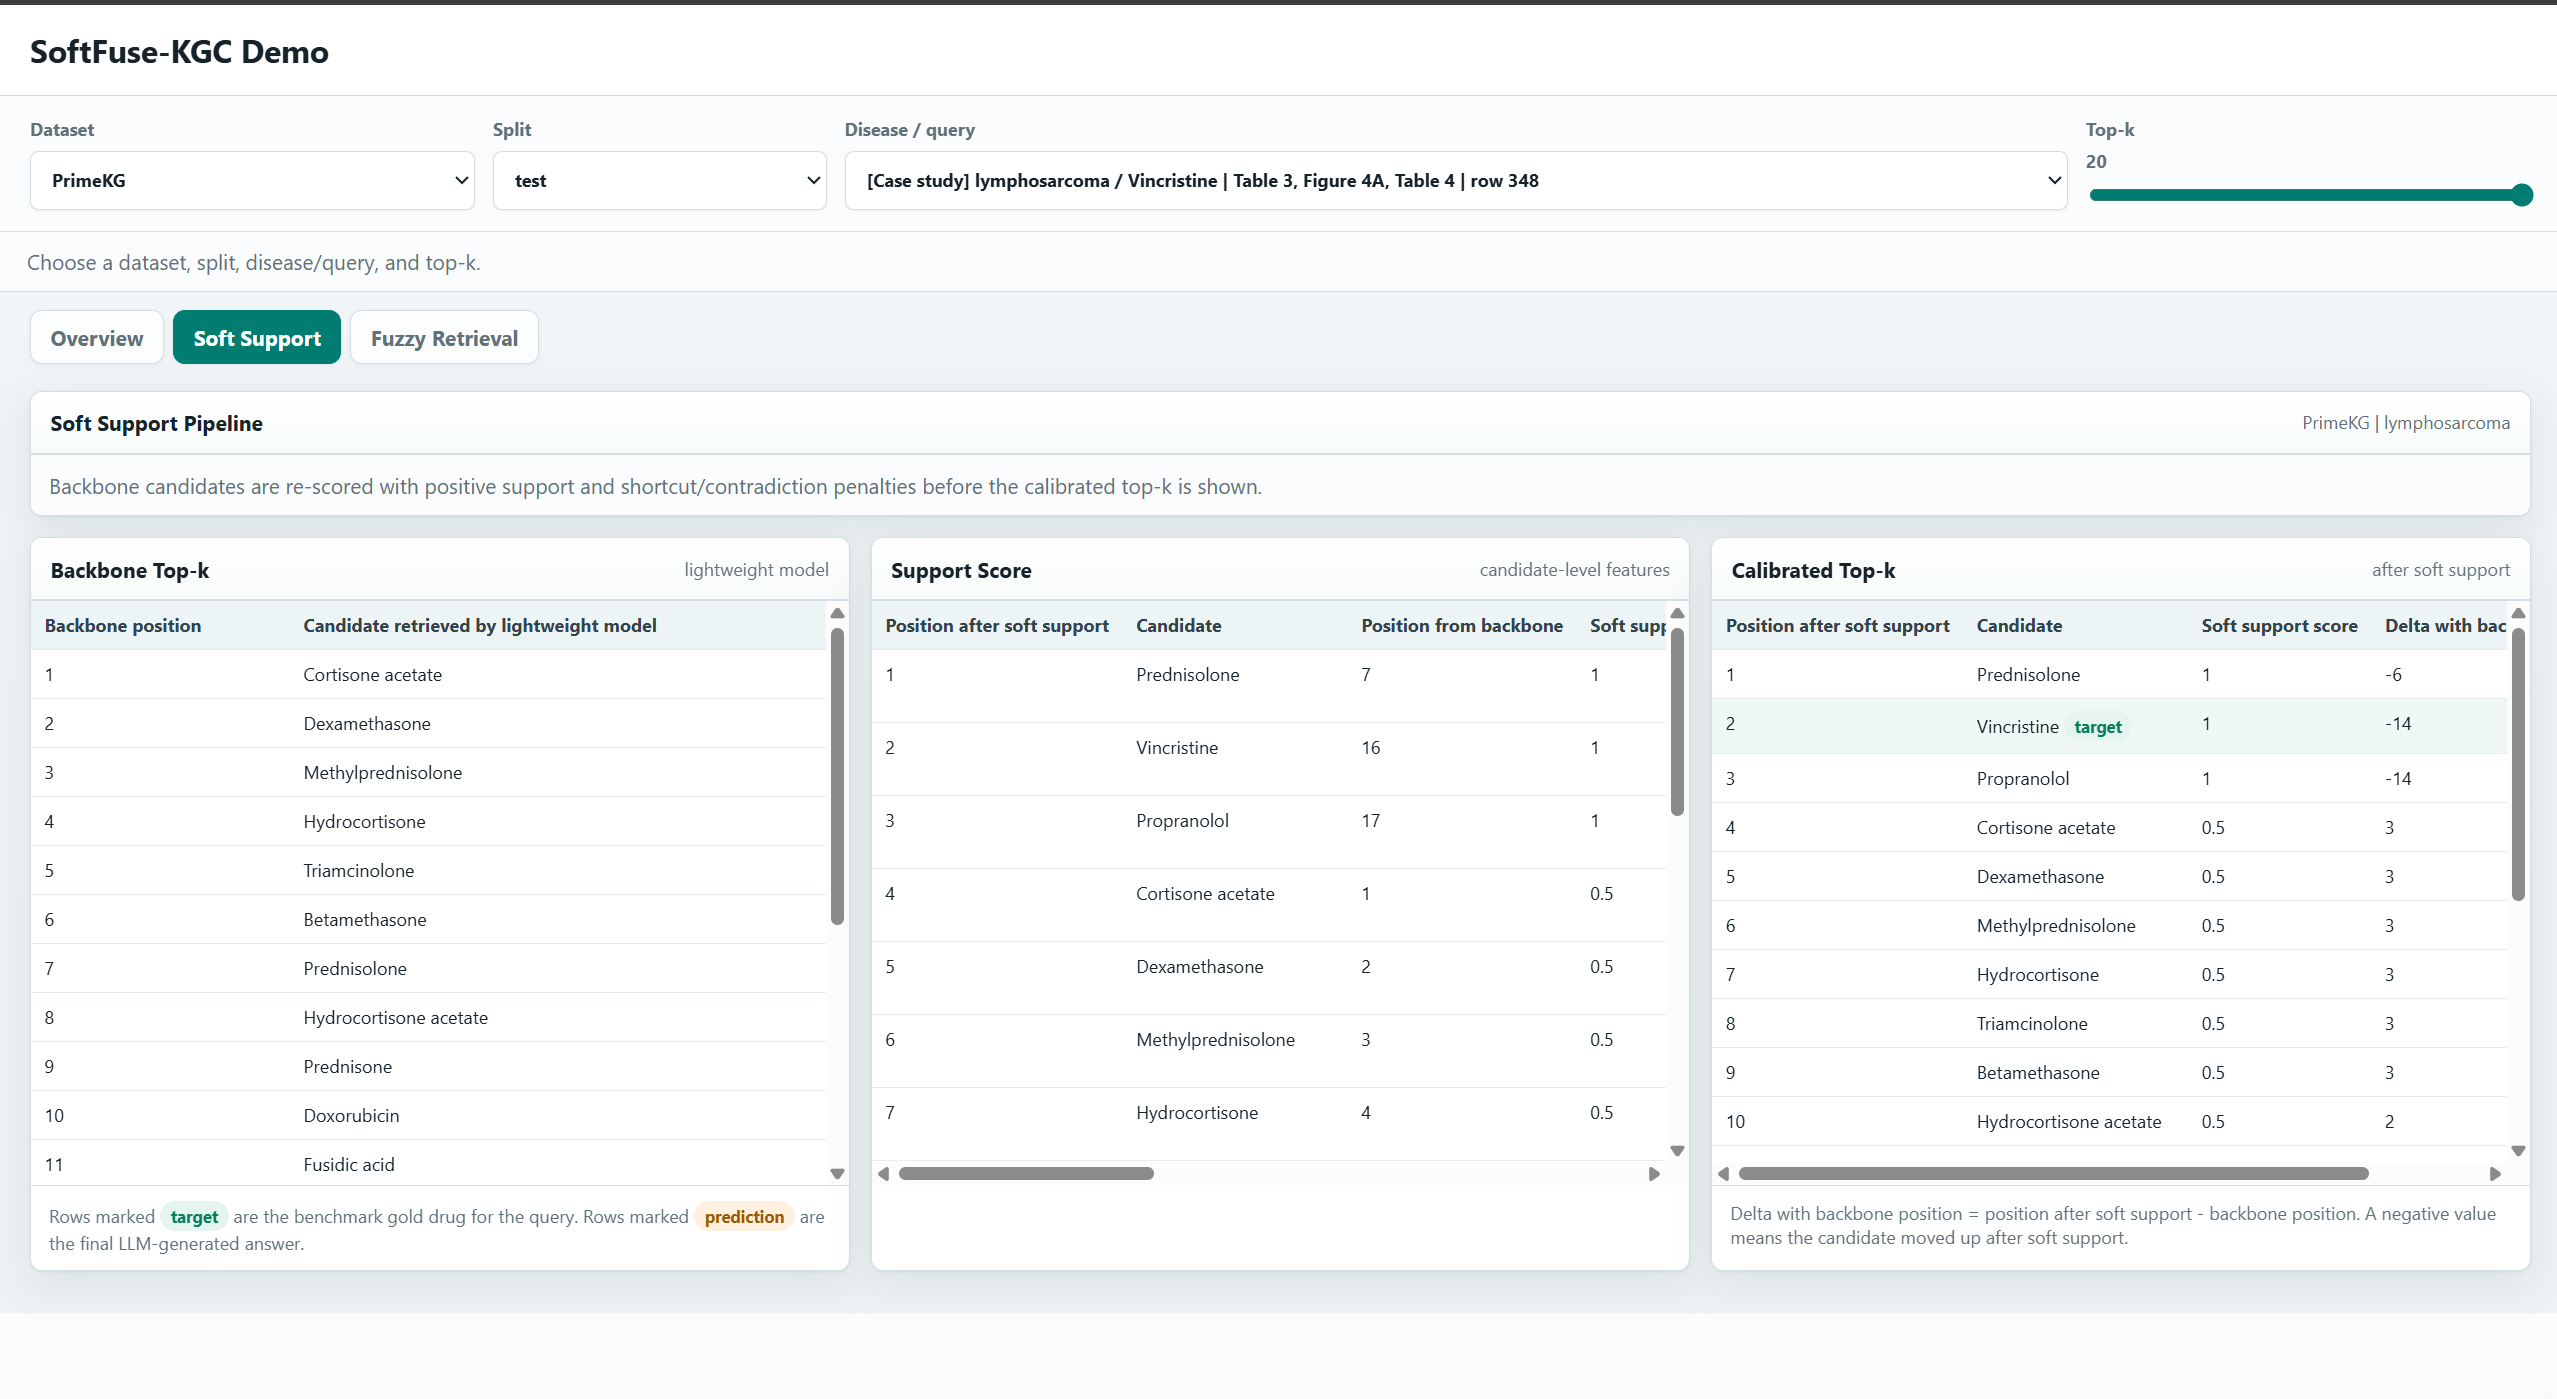
\includegraphics[width=\textwidth]{FigS2.png}
    \caption{\textbf{Soft Support tab.} The left panel reports the original lightweight-backbone top-\(k\) order. The center panel shows the final support score and available feature terms, including positive evidence, shared-gene or bridge evidence, and shortcut or contradiction penalties. The right panel gives the calibrated top-\(k\). ``Delta with backbone position'' is calibrated rank minus backbone rank; negative values indicate upward movement}
    \label{fig:s2_soft_support}
    \end{figure}

    \begin{figure}[H]
    \centering
    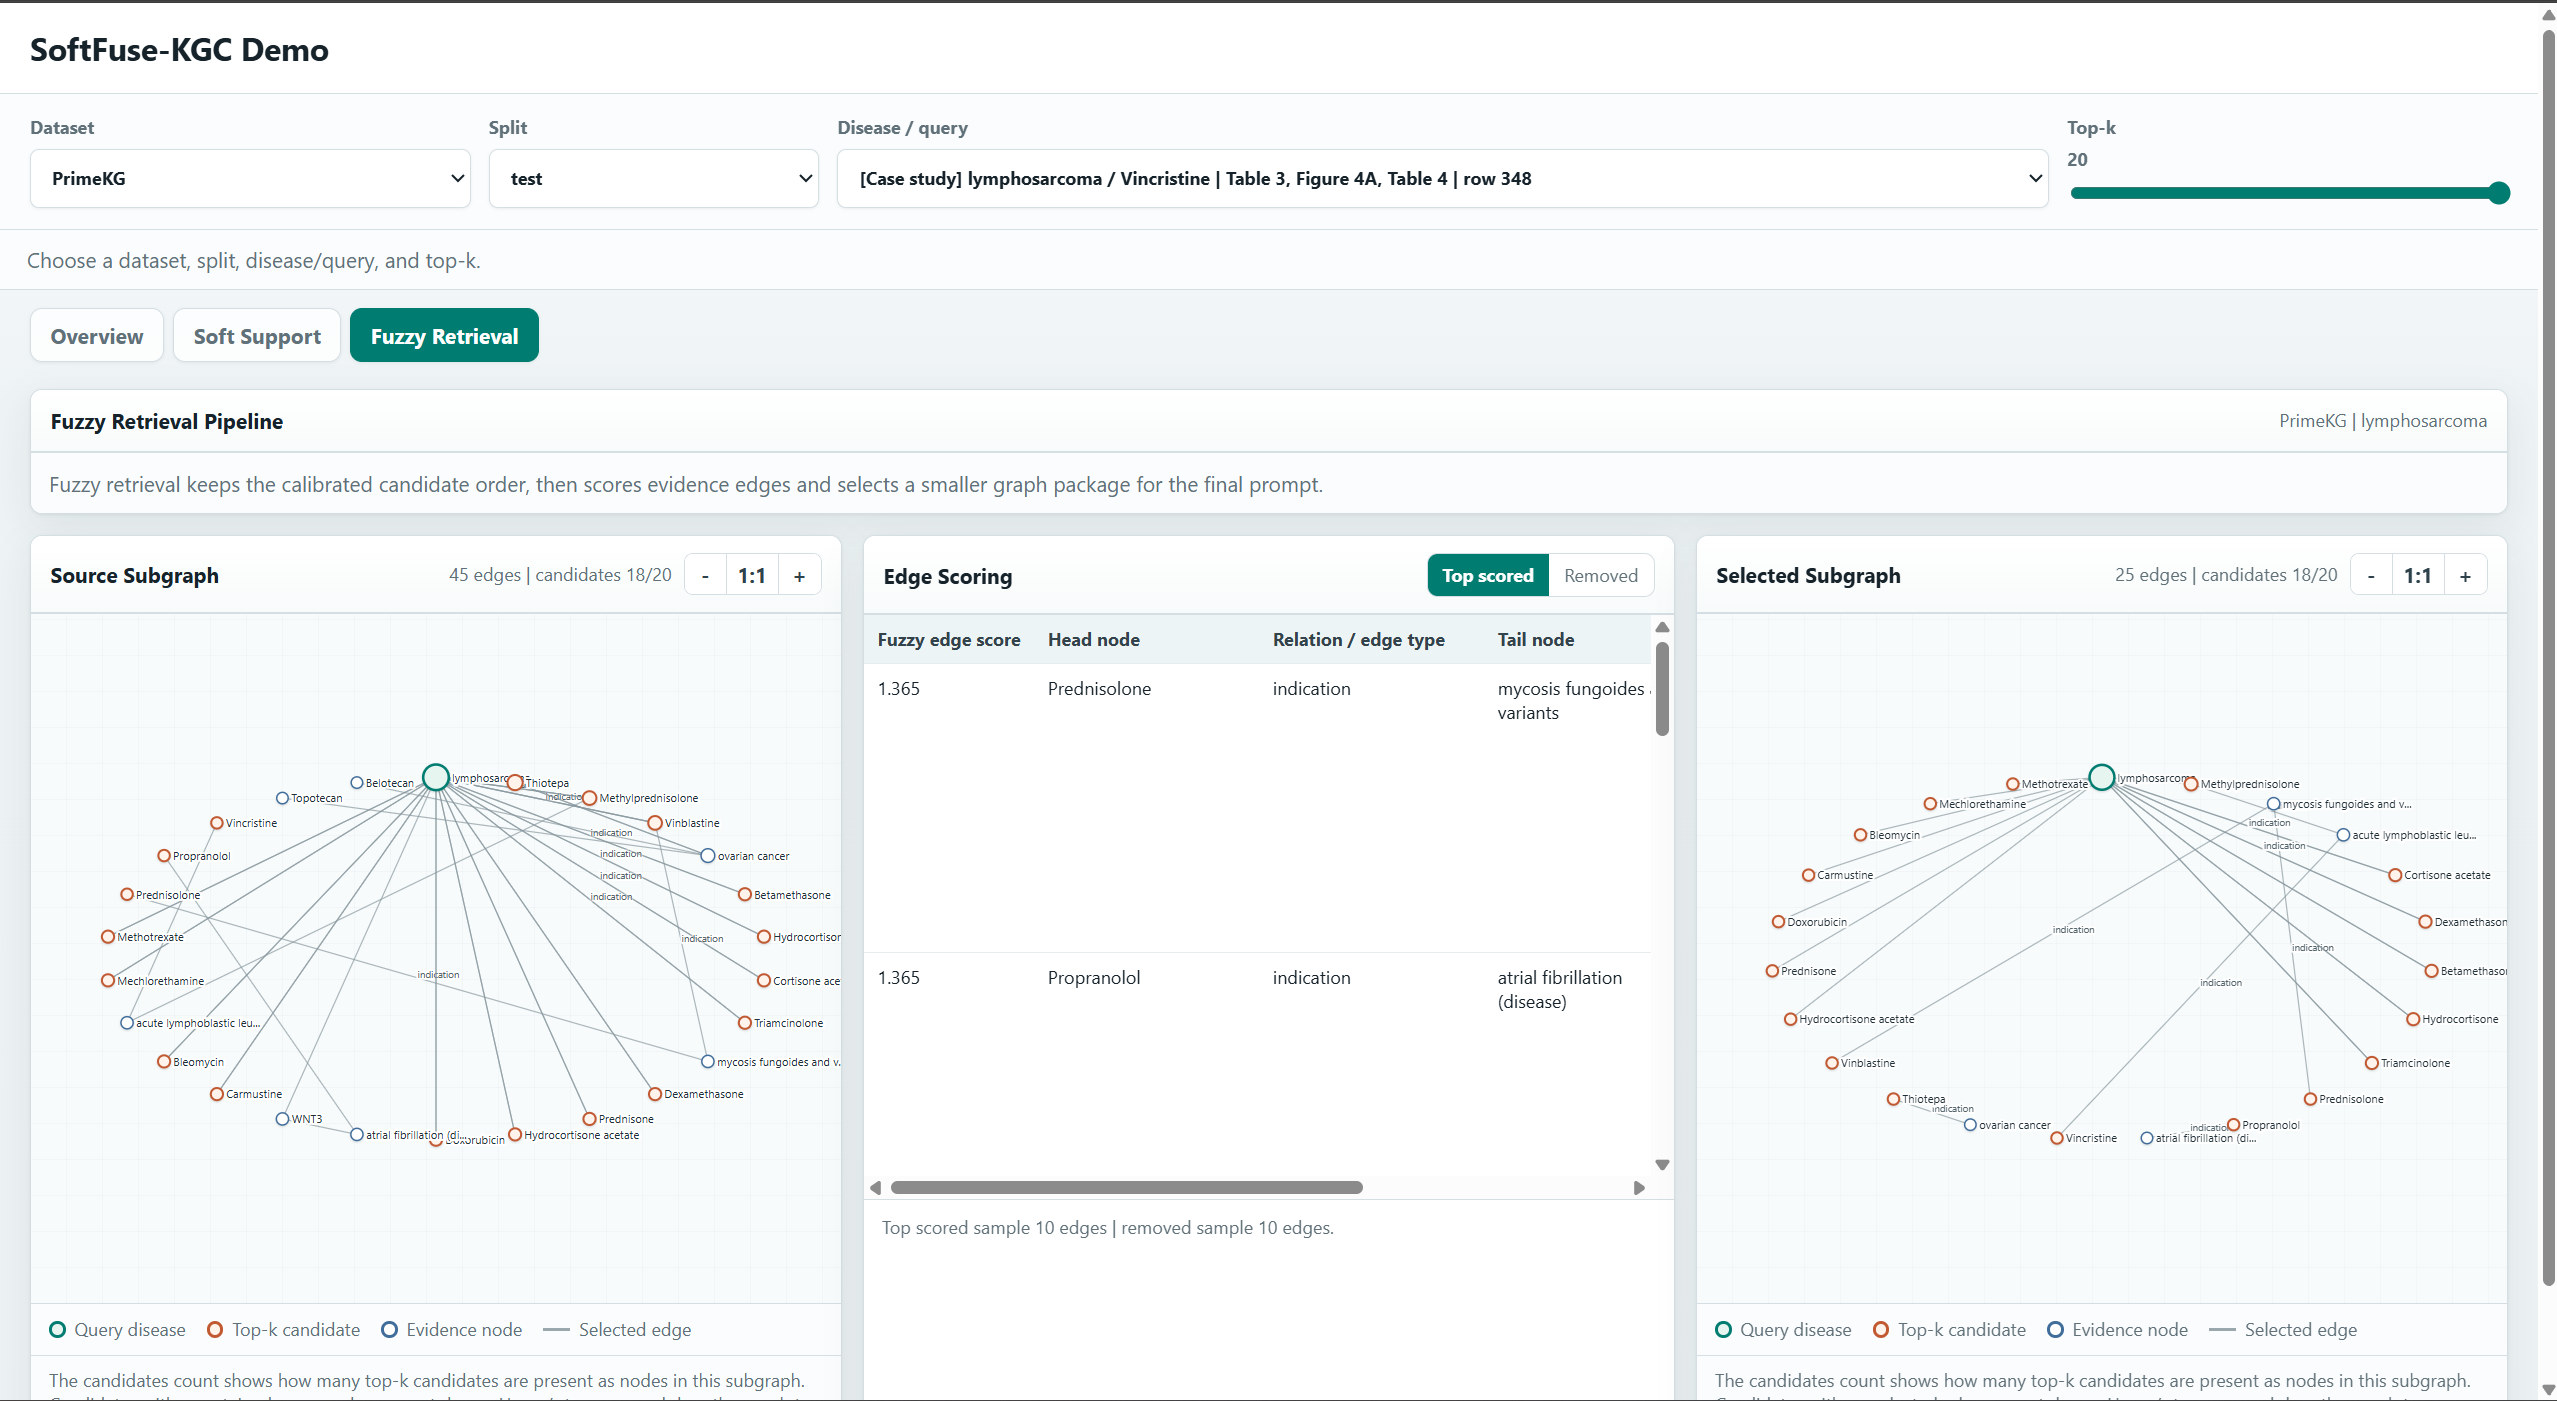
\includegraphics[width=\textwidth]{FigS3.png}
    \caption{\textbf{Fuzzy Retrieval tab.} The left panel reports the source subgraph, source-edge count, and candidate coverage. The center panel lists fuzzy edge scores and their component terms and can show either retained or removed evidence. The right panel shows the selected compact subgraph. Labels and the legend identify the query disease, top-\(k\) candidates, evidence nodes, and selected edges; color is a redundant visual cue. Zoom, reset, and drag controls support inspection}
    \label{fig:s3_fuzzy_retrieval}
    \end{figure}

    \section{Soft-Support Feature and Weight Assignment}

    Equation numbers in this Online Resource refer to the corresponding equations in the main article.

    \[
    \begin{aligned}
    \text{Eq. (2):}\quad
    E_i(q)&=\omega_{\mathrm{touch}}T_i(q)+\omega_{\mathrm{path}}P_i(q)
    +\omega_{\mathrm{schema}}A_i(q)+\omega_{\mathrm{density}}\Delta_i(q),\\
    \text{Eq. (3):}\quad
    P_i(q)&=\nu_sM^s_i(q)+\nu_bM^b_i(q)\\
    &+\nu_cT^c_i(q)+\nu_qT^q_i(q),\\
    M^s_i(q)&=\min\!\left(1,\frac{|G(c_i)\cap G(q)|}{\eta_s}\right),\\
    M^b_i(q)&=\min\!\left(1,\frac{B_i(q)}{\eta_b}\right),\\
    \text{Eq. (5):}\quad
    \Delta_i(q)&=\min\!\left(1,\frac{\log(1+\deg_{S^{(0)}_q}(c_i)+\deg_{S^{(0)}_q}(t_q))}{\eta_\Delta}\right),\\
    \text{Eq. (6):}\quad
    D_i(q)&=\max\!\left(\mathbb{I}[c_i\leftrightarrow t_q\ \text{in}\ S^{(0)}_q],
    \min\!\left(1,\frac{\deg_{\mathrm{direct}}(c_i)}{\eta_D}\right)\right),\\
    \text{Eq. (7):}\quad
    X_i(q)&=\mathbb{I}[c_i\leftrightarrow t_q\ \text{through contradiction-like evidence}],\\
    \text{Eq. (8):}\quad
    \widetilde{S}_{\theta_d}(c_i,q)&=
    \alpha_{E,d}E_i(q)-\alpha_{D,d}D_i(q)-\alpha_{X,d}X_i(q),\\
    S_{\theta_d}(c_i,q)&=\mu_dR_i(q)+(1-\mu_d)N_q(\widetilde{S}_{\theta_d}(c_i,q)).
    \end{aligned}
    \]
    When \(\mu_d>0\), the within-query normalizer in \mainequation{8} is
    \[
    N_q(z_i)=
    \begin{cases}
    \dfrac{z_i-\min_jz_j}{\max_jz_j-\min_jz_j}, & \max_jz_j>\min_jz_j,\\[0.7em]
    0.5, & \max_jz_j=\min_jz_j.
    \end{cases}
    \]

    \subsection{Feature Selection Method}

    The soft-support feature family was obtained through an audit-and-calibration procedure. First, for each validation query and each top-20 candidate, a candidate-level feature table was built from the retrieved source subgraph and the training evidence graph. The initial table included type/schema flags, ontology-support flags, candidate evidence contact, query evidence contact, direct candidate-query contact, contradiction or conflict flags, and local count features. For mechanistic datasets, the same procedure was extended to compound-gene, disease-gene, and gene-gene neighborhoods, producing shared-gene, bridge, candidate-touch, and query-touch counts.

    The candidate attributes were then summarized by frequency, value range, and gold-versus-non-gold separation. Attributes that were constant or nearly constant on the candidate set were not used as active ranking signals. Attributes that were too sparse but had a clear negative or diagnostic interpretation were retained only as small penalty channels. Attributes that appeared often enough and had an interpretable biomedical role were grouped into the general formula: \(T_i(q)\) for evidence contact, \(P_i(q)\) for mechanism-oriented support, \(A_i(q)\) for schema compatibility when informative, \(\Delta_i(q)\) for bounded local density, \(D_i(q)\) for direct shortcut or hub-like evidence, and \(X_i(q)\) for contradiction-like evidence.

    Candidate-stage formulas were then probed as simple score variants before freezing the final coefficient family. The validation rule was to preserve \gold{}, improve or maintain \mrr{}, and reduce shortcut exposure. This procedure is why the final soft-support formula separates positive evidence from direct-link penalties instead of using a hard ontology filter or a raw count score. On PrimeKG, for example, the selected contact-based b050 row improved \mrr{} to \(0.1356\), had no worsened queries relative to the backbone, and reduced the top-five direct-link rate from \(0.2408\) to \(0.0072\). The count-like capped-evidence contrast dropped to \(\mathrm{MRR@20}=0.0925\) and restored a shortcut-heavy top-five direct-link rate of \(0.2452\).

    The candidate-density feature in \mainequation{5} is retained in the general formulation because it was part of this audited feature family, but it is inactive in the reported candidate reranking rows. In the validation audit, local density behaved as a hub-sensitive count signal at the candidate stage rather than as a reliable therapeutic-support signal. It is therefore assigned zero candidate-stage weight and retained later only as a small edge-level tie breaker in \mainequation{13}.

    \subsection{Weight Assignment Method}

    Weights and normalizers were fixed using validation data only. Candidate-stage settings were retained when they preserved \gold{} and improved or maintained \mrr{} while reducing shortcut exposure. For \mainequation{3}, \(\eta_s\) and \(\eta_b\) are saturation thresholds for shared-gene and bridge counts, and \(\nu_s,\nu_b,\nu_c,\nu_q\) distribute positive support across shared-gene, bridge, candidate-touch, and query-touch channels. For Hetionet and DRKG, \(\nu_s=0.70\), \(\nu_b=0.20\), \(\nu_c=0.05\), and \(\nu_q=0.05\).

    For \mainequation{6}, \(\eta_D\) is the \(95\)th percentile of nonzero compound-to-disease direct degrees when direct-degree statistics are used. This high-percentile normalizer penalizes generic direct-disease hubs without letting a single extreme hub define the scale. Otherwise, the direct edge flag alone is used. For \mainequation{8}, \(N_q\) is the identity map when \(\mu=0\); when \(\mu>0\), the min--max rule above is applied over the 20 candidates for the same query.
    \clearpage
    \subsection{Frozen Assigned Values}

    Table~\ref{tab:s1_soft_support} reports the frozen feature instantiations, weights, and normalizers.

    \begin{table}[H]
    \caption{\textbf{Dataset-specific soft-support coefficients and feature instantiations.} These values instantiate \mainequation{2}, \mainequation{3}, \mainequation{5}, \mainequation{6}, \mainequation{7}, and \mainequation{8}.}
    \label{tab:s1_soft_support}
    \footnotesize
    \begin{tabularx}{\textwidth}{L{0.12\textwidth} Y Y Y}
    \toprule
    Dataset & Positive support instantiation & Penalty and rank-prior coefficients & Normalizers and inactive terms \\
    \midrule
    PrimeKG &
    In \mainequation{2}, \(E_i(q)\) is contact-based: \(E_i(q)=1\) when the candidate has positive evidence contact in the source subgraph and \(0\) otherwise. &
    In \mainequation{8}, \(\alpha_E=1.0\), \(\alpha_D=0.50\), \(\alpha_X=0.10\), and \(\mu=0\). In \mainequation{6}, \(D_i(q)\) is the direct candidate-query flag; in \mainequation{7}, \(X_i(q)\) uses contradiction-like evidence when available. &
    The path term in \mainequation{3}, density term in \mainequation{5}, and direct-degree normalizer in \mainequation{6} are inactive in the final candidate score. \\
    \addlinespace
    PharmKG &
    In \mainequation{2}, \(E_i(q)\) is the evidence-positive support flag for the therapeutic-association proxy relation. &
    In \mainequation{8}, \(\alpha_E=1.0\), \(\alpha_D=0.50\), \(\alpha_X=0.10\), and \(\mu=0\). In \mainequation{7}, \(X_i(q)\) is fixed to zero because no stable contradiction-like relation is used. &
    The path term in \mainequation{3}, density term in \mainequation{5}, and direct-degree normalizer in \mainequation{6} are inactive in the final candidate score. \\
    \addlinespace
    Hetionet &
    In \mainequation{3}, mechanistic support combines shared genes, gene-gene bridge evidence, candidate touch, and query touch. Candidate-gene cap \(=120\), disease-gene cap \(=300\), bridge cap \(=30\). &
    In \mainequation{8}, \(\alpha_E=1.0\), \(\alpha_D=0.50\), \(\alpha_X=0.10\), and \(\mu=0\). In \mainequation{6}, direct shortcut evidence includes direct drug-disease evidence and generic direct-disease degree. &
    In \mainequation{3}, \(\eta_s=2\), \(\eta_b=5\), \(\nu_s=0.70\), \(\nu_b=0.20\), \(\nu_c=0.05\), and \(\nu_q=0.05\). In \mainequation{6}, \(\eta_D=5.0\). The candidate-density term in \mainequation{5} is inactive. \\
    \addlinespace
    DRKG &
    In \mainequation{3}, mechanistic support combines shared genes, gene-gene bridge evidence, candidate touch, and query touch. Candidate-gene cap \(=120\), disease-gene cap \(=240\), bridge cap \(=40\). &
    In \mainequation{8}, \(\alpha_E=1.0\), \(\alpha_D=0.10\), \(\alpha_X=0.10\), and \(\mu=0.80\). The rank prior is retained because support features are sparse and hub-sensitive. &
    In \mainequation{3}, \(\eta_s=2\), \(\eta_b=6\), \(\nu_s=0.70\), \(\nu_b=0.20\), \(\nu_c=0.05\), and \(\nu_q=0.05\). In \mainequation{6}, \(\eta_D=52.95\). The candidate-density term in \mainequation{5} is inactive. \\
    \addlinespace
    repoDB &
    In \mainequation{2}, diagnostic support combines approved direct evidence, compound-gene evidence, and gene-bridge evidence:
    \(0.55\) approved direct, \(0.30\min(1,\mathrm{compound\ gene}/8)\), and \(0.15\min(1,\mathrm{gene\ bridge}/12)\). &
    In \mainequation{8}, \(\alpha_E=1.0\), \(\alpha_D=0\), \(\alpha_X=0.20\), and \(\mu=0.95\). The high rank-prior mixture reflects sparse query-specific mechanistic support in the local disease namespace. &
    The direct-degree feature in \mainequation{6} is computed but inactive because \(\alpha_D=0\). The candidate-density term in \mainequation{5} is inactive. In \mainequation{7}, the failed/diagnostic-like penalty is retained as \(X_i(q)\). \\
    \bottomrule
    \end{tabularx}
    \end{table}
    \FloatBarrier

    \section{Fuzzy Edge-Scoring Feature and Weight Assignment}

    \[
    \begin{aligned}
    \text{Eq. (10):}\quad
    B(e,q)&=\max_{c_i\in C^{\mathrm{in}}_q: e\sim c_i}w_b(r_i),\\
    w_b(r_i)&=
    \begin{cases}
    1.00, & 1\le r_i\le5,\\
    0.60, & 6\le r_i\le10,\\
    0.25, & 11\le r_i\le20,
    \end{cases}
    \end{aligned}
    \]
    \[
    \begin{aligned}
    \text{Eq. (11):}\quad
    S_{\mathrm{edge}}(e,q)&=
    \lambda_fF_r(e)+\lambda_bB(e,q)+\lambda_cT^c_e(q)\\
    &+\lambda_qT^q_e(q)+\lambda_{\mathrm{top}}H_e(q)-\lambda_dD_e(q)\\
    &-\lambda_xX_e(q)+\lambda_\rho\rho_e(q),\\
    \text{Eq. (12):}\quad
    T^c_e(q)&=\mathbb{I}[e\ \text{touches at least one candidate}],\\
    T^q_e(q)&=\mathbb{I}[e\ \text{touches the query entity}],\\
    H_e(q)&=\mathbb{I}[e\ \text{touches a top-band candidate}],\\
    \text{Eq. (13):}\quad
    \rho_e(q)&=\frac{\log(1+\deg_{S^{(0)}_q}(u))+\log(1+\deg_{S^{(0)}_q}(v))}{\eta_\rho}.
    \end{aligned}
    \]

    \subsection{Feature Selection Method}

    The fuzzy-retrieval feature family was selected after the candidate order had been fixed. The first step was to convert each retrieved source subgraph into a triple-level feature table. For each evidence triple, the audit recorded whether it touched a candidate, which candidate rank band it touched, whether it touched a top-band candidate, whether it touched the query entity, whether it formed a direct candidate-query shortcut, whether it inherited a contradiction-like flag, its relation family when relation labels were stable, and a bounded local-density hint.

    These triple attributes were summarized by occurrence frequency and by their effect on coverage-preserving graph compression. Features were retained when they controlled one of the retrieval decisions needed by the fuzzy package: preserving candidate and query anchoring, transferring confidence from the fixed candidate ranking, prioritizing interpretable biomedical relation families, demoting direct or negative-like shortcut evidence, or breaking ties among otherwise comparable triples. This audit produced the candidate-band score \(B(e,q)\), incidence indicators \(T^c_e(q)\) and \(T^q_e(q)\), the top-candidate indicator \(H_e(q)\), relation-family priority \(F_r(e)\), shortcut and contradiction penalties \(D_e(q),X_e(q)\), and the density term \(\rho_e(q)\).

    The resulting features were then tested in coverage-then-fill retrieval variants. A feature combination was kept only if the selected graph preserved the candidate order, \gold{}, candidate \mrr{}, and candidate coverage while reducing the average evidence package or lowering shortcut-heavy evidence. On the PrimeKG validation audit, the selected Fuzzy-compact setting preserved the soft-support ranking metrics and candidate coverage while reducing the average subgraph from \(60.45\) to \(32.56\) triples. The intermediate Fuzzy-balanced and Fuzzy-shortcut variants retained \(36.714\) triples on average. All fuzzy variants reduced direct-shortcut exposure. This is why fuzzy retrieval is treated as evidence packaging rather than as a second candidate reranker.

    \subsection{Weight Assignment Method}

    Fuzzy edge weights were fixed on validation data after the input candidate order had already been selected. Eligible settings had to preserve \gold{} and candidate \mrr{}, maintain candidate coverage, and reduce or clean the evidence graph. Candidate rank bands are assigned after the top-20 list is fixed: ranks \(1\)--\(5\) receive weight \(1.00\), ranks \(6\)--\(10\) receive weight \(0.60\), and ranks \(11\)--\(20\) receive weight \(0.25\). If an edge touches multiple candidates, \mainequation{10} uses the highest touched-candidate band weight; if it touches no candidate and is not part of a candidate-anchored path, its band score is zero.

    The density term in \mainequation{13} uses \(\eta_\rho=10\) for PrimeKG, Hetionet, DRKG, and repoDB. PrimeKG uses a capped local-density hint, whereas Hetionet, DRKG, and repoDB use the log-degree density term shown above. PharmKG keeps its native local touch-count density hint. The density coefficient is \(0.05\) in the selected fuzzy rows, so density acts as a tie-breaking signal after candidate coverage, relation-family evidence, and penalty terms have been applied.

    \subsection{Frozen Assigned Values}

    Table~\ref{tab:s2_fuzzy_weights} reports the frozen edge-scoring weights.

    \[
    \begin{aligned}
    \text{Eq. (10):}\quad
    B(e,q)&=\max_{c_i\in C^{\mathrm{in}}_q: e\sim c_i}w_b(r_i),\\
    w_b(r_i)&=
    \begin{cases}
    1.00, & 1\le r_i\le5,\\
    0.60, & 6\le r_i\le10,\\
    0.25, & 11\le r_i\le20,
    \end{cases}
    \end{aligned}
    \]
    \[
    \begin{aligned}
    \text{Eq. (11):}\quad
    S_{\mathrm{edge}}(e,q)&=
    \lambda_fF_r(e)+\lambda_bB(e,q)+\lambda_cT^c_e(q)\\
    &+\lambda_qT^q_e(q)+\lambda_{\mathrm{top}}H_e(q)-\lambda_dD_e(q)\\
    &-\lambda_xX_e(q)+\lambda_\rho\rho_e(q),\\
    \text{Eq. (12):}\quad
    T^c_e(q)&=\mathbb{I}[e\ \text{touches at least one candidate}],\\
    T^q_e(q)&=\mathbb{I}[e\ \text{touches the query entity}],\\
    H_e(q)&=\mathbb{I}[e\ \text{touches a top-band candidate}],\\
    \text{Eq. (13):}\quad
    \rho_e(q)&=\frac{\log(1+\deg_{S^{(0)}_q}(u))+\log(1+\deg_{S^{(0)}_q}(v))}{\eta_\rho}.
    \end{aligned}
    \]
    
    \begin{table}[H]
    \caption{\textbf{Frozen fuzzy edge-scoring weights.} These values instantiate \mainequation{10}, \mainequation{11}, \mainequation{12}, and \mainequation{13}. All datasets use rank bands 1--5, 6--10, and 11--20 with weights \(1.0\), \(0.6\), and \(0.25\), respectively.}
    \label{tab:s2_fuzzy_weights}
    \footnotesize
    \begin{tabularx}{\textwidth}{L{0.12\textwidth} Y Y Y}
    \toprule
    Dataset & Candidate, query, and density weights & Relation-family priorities & Penalty terms \\
    \midrule
    PrimeKG &
    In \mainequation{10}--\mainequation{11}, \(\lambda_b=1.0\), \(\lambda_c=0.35\), \(\lambda_q=0.05\), \(\lambda_{\mathrm{top}}=0\), and \(\lambda_\rho=0.05\). In \mainequation{13}, density uses a capped local-density hint with \(\eta_\rho=10\). &
    In \mainequation{11}, \(\lambda_f=0\); no relation-family priority is used. &
    In \mainequation{11}, the direct shortcut penalty is \(\lambda_d=0.80\), and the contradiction penalty is \(\lambda_x=0.10\). \\
    \addlinespace
    PharmKG &
    In \mainequation{10}--\mainequation{11}, \(\lambda_b=1.0\), \(\lambda_c=0.35\), \(\lambda_q=0.05\), \(\lambda_{\mathrm{top}}=0\), and \(\lambda_\rho=0.05\). The density term keeps the native local touch-count hint. &
    In \mainequation{11}, \(\lambda_f=0\); no relation-family priority is used. &
    In \mainequation{11}, the direct shortcut penalty is \(\lambda_d=0.80\), and the contradiction penalty is \(\lambda_x=0\). \\
    \addlinespace
    Hetionet &
    In \mainequation{10}--\mainequation{13}, \(\lambda_b=1.0\), \(\lambda_c=0.35\), \(\lambda_q=0.10\), \(\lambda_{\mathrm{top}}=0.05\), \(\lambda_\rho=0.05\), and \(\eta_\rho=10\). &
    In \mainequation{11}, \(\lambda_f=1.0\); \(F_r(e)\) is compound-gene \(0.30\), disease-gene \(0.30\), gene-gene \(0.20\), direct drug-disease \(0.05\), or other \(0.05\). &
    In \mainequation{11}, \(\lambda_d=0.50\) and \(\lambda_x=0\). \\
    \addlinespace
    DRKG &
    In \mainequation{10}--\mainequation{13}, \(\lambda_b=1.0\), \(\lambda_c=0.35\), \(\lambda_q=0.10\), \(\lambda_{\mathrm{top}}=0.05\), \(\lambda_\rho=0.05\), and \(\eta_\rho=10\). &
    In \mainequation{11}, \(\lambda_f=1.0\); \(F_r(e)\) is compound-gene \(0.30\), disease-gene \(0.30\), gene-gene \(0.20\), target-treats \(0.05\), auxiliary compound-disease \(0.05\), or other \(0.05\). &
    In \mainequation{11}, \(\lambda_d=0.50\) and \(\lambda_x=0\). \\
    \addlinespace
    repoDB &
    In \mainequation{10}--\mainequation{13}, \(\lambda_b=1.0\), \(\lambda_c=0.35\), \(\lambda_q=0.10\), \(\lambda_{\mathrm{top}}=0.05\), \(\lambda_\rho=0.05\), and \(\eta_\rho=10\). &
    In \mainequation{11}, \(\lambda_f=1.0\); \(F_r(e)\) is target-approved \(0.10\), failed-diagnostic \(0.02\), compound-gene \(0.35\), gene-gene \(0.25\), other compound-disease \(0.05\), or other \(0.05\). &
    In \mainequation{11}, \(\lambda_d=0.40\) and \(\lambda_x=0.15\) for failed-diagnostic evidence. \\
    \bottomrule
    \end{tabularx}
    \end{table}
    \FloatBarrier

    \clearpage

    \section{Fuzzy Retrieval Budgets}

    \[
    \begin{aligned}
    S^{\mathrm{fuzzy}}_q&=
    \operatorname{TopEdges}\!\left(S^{(0)}_q,S_{\mathrm{edge}},\tau_{d,q}\right), &&\text{\mainequation{14}}\\
    C^{\mathrm{fuzzy}}_q&=C^{\mathrm{in}}_q. &&\text{\mainequation{15}}
    \end{aligned}
    \]

    The budget values in Table~\ref{tab:s3_fuzzy_budgets} instantiate \mainequation{14}, while \mainequation{15} fixes the candidate order after fuzzy graph selection.

    \begin{table}[H]
    \caption{\textbf{Frozen fuzzy retrieval budgets and coverage checks.} These settings instantiate the graph budget \(\tau_{d,q}\) in \mainequation{14}; candidate rankings are preserved as in \mainequation{15}.}
    \label{tab:s3_fuzzy_budgets}
    \footnotesize
    \begin{tabularx}{\textwidth}{L{0.12\textwidth} Y Y Y}
    \toprule
    Dataset & Budget rule & Selection passes & Frozen coverage result \\
    \midrule
    PrimeKG &
    In \mainequation{14}, retain ratio \(0.55\), minimum \(18\), maximum equal to source size. &
    Candidate coverage pass, then global fill by edge score. &
    Validation \(60.45\rightarrow32.56\) triples; test \(59.93\rightarrow32.34\) triples. Candidate coverage preserved: \(1.0\). \\
    \addlinespace
    PharmKG &
    In \mainequation{14}, retain ratio \(0.55\), minimum \(18\), maximum equal to source size. &
    Candidate coverage pass, then global fill by edge score. &
    Validation and test \(100\rightarrow55\) triples. Candidate, top-band, middle-band, and tail-band coverage preserved: \(1.0\). \\
    \addlinespace
    Hetionet &
    In \mainequation{14}, retain ratio \(0.55\), minimum \(28\), maximum \(48\). &
    Candidate coverage pass, query coverage pass, then global fill. &
    Validation and test \(80\rightarrow44\) triples. Candidate coverage preserved: \(1.0\). \\
    \addlinespace
    DRKG &
    In \mainequation{14}, retain ratio \(0.55\), minimum \(45\), maximum \(60\), family minimum \(3\). &
    Candidate coverage pass, query coverage pass, family preservation pass, then global fill. &
    Validation and test \(100\rightarrow55\) triples. Candidate coverage preserved: \(1.0\). \\
    \addlinespace
    repoDB &
    In \mainequation{14}, retain ratio \(0.55\), minimum \(45\), maximum \(60\). Family minimums are compound-gene \(8\), gene-gene \(6\), target \(1\), and failed \(0\). &
    Candidate coverage pass, query coverage pass, family preservation pass, then global fill. &
    Validation and test \(100\rightarrow55\) triples. Candidate coverage preserved: \(1.0\). \\
    \bottomrule
    \end{tabularx}
    \end{table}
    \FloatBarrier

    \section{Algorithm}

    \[
    \begin{aligned}
    S_{\theta_d}(c_i,q)&=\mu_dR_i(q)+(1-\mu_d)N_q(\widetilde{S}_{\theta_d}(c_i,q)), &&\text{\mainequation{8}}\\
    c_i\prec c_j&\Longleftrightarrow S_i>S_j\ \mathrm{or}\ (S_i=S_j\ \mathrm{and}\ r_i^{(0)}<r_j^{(0)}), &&\text{\mainequation{9}}\\
    S_{\mathrm{edge}}(e,q)&=
    \lambda_fF_r(e)+\lambda_bB(e,q), &&\text{\mainequation{11}}\\
    &\quad+\lambda_cT^c_e(q)+\lambda_qT^q_e(q)+\lambda_{\mathrm{top}}H_e(q)\\
    &\quad-\lambda_dD_e(q)-\lambda_xX_e(q)+\lambda_\rho\rho_e(q),\\
    S^{\mathrm{fuzzy}}_q&=
    \operatorname{TopEdges}\!\left(S^{(0)}_q,S_{\mathrm{edge}},\tau_{d,q}\right), &&\text{\mainequation{14}}\\
    \mathbf{z}_e&=
    \mathrm{Adapter}\left([\mathbf{h}^{\mathrm{global}}_e;\mathbf{h}^{\mathrm{local}}_e]\right). &&\text{\mainequation{16}}
    \end{aligned}
    \]

    Algorithm~\ref{alg:supp_softfuse} summarizes the complete inference sequence for one query.

    \begin{algorithm}[H]
    \footnotesize
    \caption{\softfuse{} inference for one query}
    \label{alg:supp_softfuse}
    \begin{algorithmic}[1]
    \REQUIRE Query \(q=(?,r_q,t_q)\), candidate universe \(\mathcal{C}_d\), graph-compatible ranker, source graph retriever, support features, edge score \(S_{\mathrm{edge}}\)
    \STATE Retrieve the initial top-20 candidate list \(C_q^{(0)}\).
    \STATE Build the source evidence subgraph \(S_q^{(0)}\) from the query, candidates, and available rule/path evidence.
    \STATE Compute candidate support scores \(S_{\theta_d}(c_i,q)\) using \mainequation{8}.
    \STATE Re-rank candidates with the tie-breaking rule in \mainequation{9} to obtain \(C_q^{\mathrm{soft}}\).
    \STATE Assign candidate bands from \(C_q^{\mathrm{soft}}\) and score evidence triples with \mainequation{11}.
    \STATE Select \(S_q^{\mathrm{fuzzy}}\) using the coverage and fill passes in Table~\ref{tab:s3_fuzzy_budgets}.
    \STATE Compute graph-enhanced query and candidate embeddings with the graph adapter in \mainequation{16}.
    \STATE Insert \texttt{[QUERY]} and \texttt{[ENTITY]} embeddings into the candidate-constrained LLM prompt.
    \STATE Generate the final answer from the calibrated candidate list.
    \RETURN Prediction \(\hat{y}_q\).
    \end{algorithmic}
    \end{algorithm}
    \FloatBarrier

    \section{Dataset Implementation Details}

    The end-to-end implementation uses a reproduced \drkgc{}-style graph-LLM setup: a graph-compatible R-GCN source provides candidate identifiers, local subgraphs, and structural embeddings for the graph adapter; the LLM is fine-tuned with LoRA; validation and test use \(K=20\) candidates. The primary dataset runs use Llama-3.2-3B with LoRA \(r=32\), \(\alpha=32\), dropout \(0.1\), learning rate \(2\times10^{-4}\), source/target lengths \(768/64\), deterministic one-beam decoding without sampling, and a single NVIDIA RTX 4090 GPU with 24GB memory. Table~\ref{tab:s4_graph_llm_implementation} reports the dataset-specific graph sources and frozen generation settings. These graph-adapter pipeline sources are distinct from the separately trained structure-only baselines reported later; their embedding dimensions therefore need not match.

    \begin{table}[H]
    \caption{\textbf{Graph-LLM implementation and decoding settings.} Common LoRA, decoding, and hardware settings are stated in the paragraph above.}
    \label{tab:s4_graph_llm_implementation}
    \footnotesize
    \setlength{\tabcolsep}{3.2pt}
    \renewcommand{\arraystretch}{1.04}
    \begin{tabularx}{\textwidth}{L{0.12\textwidth} Y Y Y}
    \toprule
    Dataset & Graph source & Training detail & Frozen decoding and graph size \\
    \midrule
    PrimeKG &
    R-GCN; \(4\) rel.; \(10453\times256\) embeddings. &
    Batch \(1\); grad. acc. \(8\). &
    New \(16\); rep. \(1.00\); no-repeat \(0\); graph \(59.93\rightarrow32.34\). \\
    PharmKG &
    R-GCN; \(28\) rel.; \(7247\times128\) embeddings. &
    Batch \(1\); grad. acc. \(16\). &
    New \(16\); rep. \(1.05\); no-repeat \(0\); graph \(100\rightarrow55\). \\
    Hetionet &
    R-GCN-compatible; \(24\) rel.; \(47031\times128\) embeddings. &
    Batch \(1\); grad. acc. \(8\). &
    New \(16\); one beam; no sampling; graph \(80\rightarrow44\). \\
    DRKG &
    R-GCN consistency source; \(85\) rel.; R-GCN-ready IDs. &
    Batch \(1\); grad. acc. \(8\). &
    New \(16\); one beam; no sampling; graph \(100\rightarrow55\). \\
    repoDB &
    R-GCN; \(63\) rel.; readable names plus canonical IDs. &
    Batch \(1\); grad. acc. \(8\). &
    New \(16\); one beam; no sampling; graph \(100\rightarrow55\). \\
    \bottomrule
    \end{tabularx}
    \end{table}
    \FloatBarrier

    Table~\ref{tab:s5_prompt_rules} lists the question templates and evidence-path retrieval packages used for each dataset.

    \begin{table}[H]
    \caption{\textbf{Pre-specified question templates and evidence-path retrieval rules.} Task templates and retrieval rules format candidate-constrained prompts and package local evidence.}
    \label{tab:s5_prompt_rules}
    \footnotesize
    \setlength{\tabcolsep}{3.2pt}
    \renewcommand{\arraystretch}{1.04}
    \begin{tabularx}{\textwidth}{L{0.12\textwidth} Y Y}
    \toprule
    Dataset & Question template & Path-rule or retrieval package \\
    \midrule
    PrimeKG &
    \emph{What drug is indicated for \{disease\}?} &
    Drug--target--gene--disease and drug--target--gene--ppi--gene--disease paths; contraindication-like drug--disease evidence is retained as a negative/safety cue. \\
    PharmKG &
    \emph{What drug is therapeutically associated with \{disease\}?} &
    The \(T\) relation is the therapeutic-association proxy; retrieval uses incident-edge and shortest-path fallback evidence. \\
    Hetionet &
    \emph{What compound treats \{disease\}?} &
    \(\mathrm{CbG}\)--\(\mathrm{DaG}\), \(\mathrm{CdG}\)--\(\mathrm{DdG}\), \(\mathrm{CuG}\)--\(\mathrm{DuG}\), one-hop \(\mathrm{GiG}\) bridges, and direct \(\mathrm{CpD}\) evidence. \\
    DRKG &
    \emph{What compound treats \{disease\}?} &
    Compound:Gene--Gene:Disease, direct Compound:Disease, and Gene:Gene bridge evidence for the DrugBank treats head-prediction target. \\
    repoDB &
    \emph{What drug is approved for \{disease\}?} &
    Compound:Gene--Gene:Gene, Compound:Disease, and failed-diagnostic evidence retained as diagnostic rather than positive approved-indication context. \\
    \bottomrule
    \end{tabularx}
    \end{table}
    \FloatBarrier

    \subsection{Prompt and Output Example}

    All datasets use the same candidate-constrained prompt pattern. The following PrimeKG example illustrates the input schema and supervised output:

    \begin{center}
    {\setlength{\fboxsep}{6pt}
    \fbox{\begin{minipage}{0.94\textwidth}
    \footnotesize
    You are a biomedical scientist. The task is to predict the answer based on the given question, and you only need to answer one entity. The answer must be in ('Fusidic acid', 'Cortisone acetate', 'Hydrocortisone', 'Betamethasone', 'Tetracycline', 'Ofloxacin', 'Ciprofloxacin', 'Demeclocycline', 'Dexamethasone', 'Triamcinolone', 'Prednisolone', 'Methylprednisolone', 'Hydrocortisone acetate', 'Methdilazine', 'Norfloxacin', 'Doxycycline', 'Prednisone', 'Alimemazine', 'Doxylamine', 'Phenylephrine').

    You can refer to the entity embeddings: 'allergic rhinitis': \texttt{[QUERY]}, 'Fusidic acid': \texttt{[ENTITY]}, 'Cortisone acetate': \texttt{[ENTITY]}, 'Hydrocortisone': \texttt{[ENTITY]}, \ldots, 'Phenylephrine': \texttt{[ENTITY]}.

    Question: What drug is indicated for allergic rhinitis?

    Answer:
    \end{minipage}}}
    \end{center}

    The corresponding supervised output is \emph{Hydrocortisone}. During evaluation, the generated string is normalized and matched against the supplied candidate list; unmatched strings are counted as invalid predictions.

    \section{PrimeKG Variant Formulas}

    PrimeKG is used here as the representative formula summary.

    \subsection{Soft-Support Variants}

    \[
    \begin{aligned}
    \text{Selected family:}\quad
    \widetilde{S}(c_i,q)&=\alpha_EE_i(q)-\alpha_DD_i(q)-\alpha_XX_i(q),\\
    \mathrm{b025}:&\quad E_i(q)-0.25D_i(q)-0.05X_i(q),\\
    \mathrm{b050}:&\quad E_i(q)-0.50D_i(q)-0.10X_i(q),\\
    \mathrm{bcap}:&\quad \min(E^{\mathrm{count}}_i(q),2)-0.50D_i(q)-0.10X_i(q).
    \end{aligned}
    \]
    The selected PrimeKG contact-support family is a special case of \mainequation{8} with \(\mu=0\). The final row uses b050. The b025 row tied b050 in validation, but b050 was retained because it applies the stronger shortcut penalty while preserving the same candidate ranking. The capped-evidence contrast underperformed because it reintroduced shortcut-heavy candidates.

    \subsection{Fuzzy-Retrieval Variants}

    \[
    S_{\mathrm{edge}}(e,q)=
    B(e,q)+0.35T^c_e(q)+0.05T^q_e(q)
    -\lambda_dD_e(q)-0.10X_e(q)+0.05\rho_e(q).
    \]
    The PrimeKG fuzzy edge score uses \mainequation{11} with no relation-family term. The selected Fuzzy-compact variant (called \emph{tight} in the configuration audit) sets \(\lambda_d=0.80\), retain ratio \(0.55\), and minimum keep \(18\). The Fuzzy-shortcut contrast (called \emph{directplus} in the audit) sets \(\lambda_d=1.00\), retain ratio \(0.67\), and minimum keep \(20\). Both preserve candidate ranking, but Fuzzy-compact gives the smaller and cleaner graph package on validation. Table~\ref{tab:s6_primekg_variants} summarizes the selected and contrastive PrimeKG rows.

    \begin{table}[H]
    \caption{\textbf{PrimeKG variant-selection summary.} Candidate metrics are validation metrics for soft support and held-out test metrics for the locked ablation rows.}
    \label{tab:s6_primekg_variants}
    \footnotesize
    \begin{tabularx}{\textwidth}{L{0.25\textwidth} c c c c Y}
    \toprule
    Row & \gold{} & \mrr{} & Hits@1 & \hitsten{} & Selection note \\
    \midrule
    Backbone raw, validation & 0.202 & 0.0918 & 0.024 & 0.158 & Reference candidate order. \\
    Ontology hard filter, validation & 0.014 & 0.0509 & 0.002 & 0.012 & Negative control; brittle under missing evidence. \\
    Soft support b050, validation & 0.202 & 0.1356 & 0.056 & 0.182 & Selected soft-support row. \\
    Capped-evidence contrast, validation & 0.202 & 0.0925 & 0.022 & 0.158 & Retained only as a contrast row. \\
    Backbone raw, test & 0.240 & 0.0646 & 0.024 & 0.192 & Locked test reference. \\
    Soft support, test & 0.240 & 0.1253 & 0.072 & 0.222 & Candidate-stage gain. \\
    Fuzzy retrieval, test & 0.240 & 0.1253 & 0.072 & 0.222 & Candidate order preserved; graph \(59.93\rightarrow32.34\). \\
    \bottomrule
    \end{tabularx}
    \end{table}
    \FloatBarrier

    \section{LLM Model Comparison}

    The model comparisons use candidate-constrained evaluation: generated strings are normalized against the supplied candidate list, and invalid outputs receive zero reciprocal rank. Table~\ref{tab:s7_primekg_llm_compare} reports the PrimeKG generator comparison.

    \begin{table}[H]
    \caption{\textbf{PrimeKG LLM comparison on the fuzzy retrieval row.} All rows use the same candidate list and fuzzy evidence package. The configuration column reports max new tokens / repetition penalty / no-repeat n-gram size.}
    \label{tab:s7_primekg_llm_compare}
    \footnotesize
    \setlength{\tabcolsep}{3.0pt}
    \renewcommand{\arraystretch}{1.04}
    \begin{tabularx}{\textwidth}{L{0.18\textwidth} c c c c c c Y}
    \toprule
    Model & Config & E2E \mrr{} & E2E \hitsten{} & Pred. in cand. & Invalid & Top1 copy & Interpretation \\
    \midrule
    Llama-3.2-3B & \(16/1.00/0\) & 0.0747 & 0.218 & 0.998 & 0.002 & 0.010 & Primary generator; high candidate validity without top-ranked candidate copying. \\
    Llama-3-8B & \(16/1.00/0\) & 0.1253 & 0.222 & 1.000 & 0.000 & 1.000 & Diagnostic generator behavior; all test outputs follow the first candidate. \\
    MedLlama-3-8B & \(16/1.00/0\) & 0.1253 & 0.222 & 1.000 & 0.000 & 1.000 & Same candidate-order-following behavior as Llama-3-8B. \\
    \bottomrule
    \end{tabularx}
    \end{table}
    \FloatBarrier

    Table~\ref{tab:s8_pharmkg_llm_compare} reports the corresponding PharmKG comparison.

    \begin{table}[H]
    \caption{\textbf{PharmKG LLM comparison on the fuzzy retrieval row.} The first three rows use the frozen PharmKG decoding configuration. Mistral-7B is included as a diagnostic comparison.}
    \label{tab:s8_pharmkg_llm_compare}
    \footnotesize
    \setlength{\tabcolsep}{3.0pt}
    \renewcommand{\arraystretch}{1.04}
    \begin{tabularx}{\textwidth}{L{0.18\textwidth} c c c c c c Y}
    \toprule
    Model & Config & E2E \mrr{} & E2E \hitsten{} & Pred. in cand. & Invalid & Top1 copy & Interpretation \\
    \midrule
    Llama-3.2-3B & \(16/1.05/0\) & 0.0210 & 0.062 & 0.412 & 0.588 & 0.412 & Most stable PharmKG generator among the frozen rows. \\
    Llama-3-8B & \(16/1.05/0\) & 0.0203 & 0.064 & 0.274 & 0.726 & 0.274 & Lower candidate validity; no PrimeKG-like top1-copy collapse. \\
    MedLlama-3-8B & \(16/1.05/0\) & 0.0186 & 0.060 & 0.022 & 0.978 & 0.022 & Mostly invalid under the candidate-constrained output rule. \\
    Mistral-7B & \(32/1.00/0\) & 0.0186 & 0.060 & 0.014 & 0.986 & 0.000 & Diagnostic comparison; candidate validity remains very low. \\
    \bottomrule
    \end{tabularx}
    \end{table}
    \FloatBarrier

    Table~\ref{tab:s8_pharmkg_llm_compare} shows a different failure mode from the PrimeKG 8B rows. Llama-3.2-3B gives the highest candidate-constrained validity on PharmKG, although invalid outputs remain frequent because the transfer task uses a noisier therapeutic-association proxy. Llama-3-8B has slightly higher \hitsten{} but lower candidate validity, while MedLlama-3-8B and Mistral-7B mostly generate strings outside the supplied candidate list.

    \subsection{Decoding-Configuration Check}

    The deterministic decoding sweep used for configuration selection varied max new tokens, repetition penalty, and no-repeat n-gram size. The sweep was performed on the validation split with the primary generator, and the selected configuration was then held fixed for the model comparison. This avoids selecting a separate decoding policy for each larger model after observing comparison outcomes. Table~\ref{tab:s9_primekg_config_audit} therefore separates two checks: the full eight-configuration sweep showing that the frozen decoding setting itself does not induce top1-copy behavior in Llama-3.2-3B, and the larger-model frozen checks showing that top1-copy appears when the generator is changed to Llama-3-8B or MedLlama-3-8B under the same selected configuration.

    \begin{table}[H]
    \caption{\textbf{PrimeKG decoding-configuration check for top1-copy behavior.} Top1-copy means that the generated entity is the first candidate in the supplied list. The Llama-3.2-3B rows report the complete validation sweep; the 8B rows report the frozen configuration used in the model comparison.}
    \label{tab:s9_primekg_config_audit}
    \footnotesize
    \setlength{\tabcolsep}{3.0pt}
    \renewcommand{\arraystretch}{1.04}
    \begin{tabularx}{\textwidth}{L{0.18\textwidth} L{0.13\textwidth} c c c L{0.13\textwidth} c c Y}
    \toprule
    Model/protocol & Config & New & Rep. & No-rep. & Val. E2E \mrr{} / \hitsten{} & Val. top1 copy & Test top1 copy & Interpretation \\
    \midrule
    Llama-3.2-3B sweep & cfg01 & 16 & 1.00 & 0 & \(0.0585/0.174\) & 0.008 & 0.010 & Frozen setting selected because all swept settings tied on the fuzzy row. \\
    Llama-3.2-3B sweep & cfg02 & 16 & 1.05 & 0 & \(0.0585/0.174\) & 0.008 & -- & Same validation metrics as cfg01. \\
    Llama-3.2-3B sweep & cfg03 & 16 & 1.10 & 0 & \(0.0585/0.174\) & 0.008 & -- & Same validation metrics as cfg01. \\
    Llama-3.2-3B sweep & cfg04 & 16 & 1.10 & 3 & \(0.0585/0.174\) & 0.008 & -- & Same validation metrics as cfg01. \\
    Llama-3.2-3B sweep & cfg05 & 24 & 1.00 & 0 & \(0.0585/0.174\) & 0.008 & -- & Same validation metrics as cfg01. \\
    Llama-3.2-3B sweep & cfg06 & 24 & 1.05 & 0 & \(0.0585/0.174\) & 0.008 & -- & Same validation metrics as cfg01. \\
    Llama-3.2-3B sweep & cfg07 & 24 & 1.10 & 0 & \(0.0585/0.174\) & 0.008 & -- & Same validation metrics as cfg01. \\
    Llama-3.2-3B sweep & cfg08 & 24 & 1.10 & 3 & \(0.0585/0.174\) & 0.008 & -- & Same validation metrics as cfg01. \\
    Llama-3-8B frozen check & cfg01 & 16 & 1.00 & 0 & \(0.0976/0.182\) & 1.000 & 1.000 & Test outputs: 464 non-gold top1 copies and 36 exact-target top1 cases. \\
    MedLlama-3-8B frozen check & cfg01 & 16 & 1.00 & 0 & \(0.0976/0.182\) & 1.000 & 1.000 & Same validation and test breakdown as Llama-3-8B. \\
    \bottomrule
    \end{tabularx}
    \end{table}
    \FloatBarrier

    The PrimeKG sweep shows that changing deterministic decoding length, repetition penalty, and no-repeat n-gram size did not change the primary generator's fuzzy-row validation metrics or create top1-copy collapse. The collapse appears only in the larger-model frozen checks, where both 8B generators copy the first candidate for every validation and test example. Their higher adjusted E2E \mrr{} is therefore interpreted as candidate-order following after the soft-support/fuzzy candidate list has already been supplied, not as stronger use of the evidence text or graph package.

    \section{Ablation, Sensitivity, and Robustness}

    Table~\ref{tab:s10_primekg_ablation} isolates the candidate-reranking and evidence-packaging contributions on the PrimeKG test split.

    \begin{table}[H]
    \caption{\textbf{PrimeKG held-out test ablation.} The soft-support row changes candidate ordering; fuzzy retrieval changes evidence packaging while preserving the candidate order.}
    \label{tab:s10_primekg_ablation}
    \footnotesize
    \begin{tabularx}{\textwidth}{L{0.22\textwidth} c c c c c Y}
    \toprule
    Row & \gold{} & \mrr{} & Hits@1 & \hitsten{} & Avg. graph & Note \\
    \midrule
    Backbone raw & 0.240 & 0.0646 & 0.024 & 0.192 & 59.93 & Initial graph-compatible source. \\
    Soft support & 0.240 & 0.1253 & 0.072 & 0.222 & 59.93 & Candidate \(\Delta\mathrm{MRR@20}=+0.0608\). \\
    Fuzzy retrieval & 0.240 & 0.1253 & 0.072 & 0.222 & 32.34 & Ranking unchanged; graph reduced by \(27.59\) triples on average. \\
    \bottomrule
    \end{tabularx}
    \end{table}
    \FloatBarrier

    Table~\ref{tab:s11_sensitivity} evaluates retrieval-rule and question-template sensitivity with a fixed candidate order.

    \begin{table}[H]
    \caption{\textbf{PrimeKG rule-package and question-template sensitivity.} Candidate order is fixed in these checks.}
    \label{tab:s11_sensitivity}
    \footnotesize
    \begin{tabularx}{\textwidth}{L{0.23\textwidth} c c c c c Y}
    \toprule
    Variant & Candidate \mrr{} & E2E \mrr{} & E2E Hits@10 & Invalid & Avg. graph & Note \\
    \midrule
    Main rules & 0.1253 & 0.0747 & 0.218 & 0.002 & 32.34 & Canonical setting. \\
    No rules & 0.1253 & 0.0747 & 0.218 & 0.020 & 59.93 & Similar rank metric but larger graph and higher invalid rate. \\
    Random rules & 0.1253 & 0.0747 & 0.218 & 0.002 & 32.34 & Diagnostic control; not selected over main rules. \\
    Canonical question & 0.1253 & 0.0747 & 0.218 & 0.002 & 32.34 & Baseline wording. \\
    Treatment wording & 0.1253 & 0.0747 & 0.218 & 0.000 & 32.34 & Prediction string changes in \(3.0\%\) of test examples. \\
    Medication wording & 0.1253 & 0.0747 & 0.218 & 0.002 & 32.34 & Prediction string changes in \(0.6\%\) of test examples. \\
    Association-neutral wording & 0.1253 & 0.0747 & 0.218 & 0.000 & 32.34 & Prediction string changes in \(4.6\%\) of test examples. \\
    \bottomrule
    \end{tabularx}
    \end{table}
    \FloatBarrier

    Table~\ref{tab:s12_noise_robustness} reports small score perturbations and edge-drop robustness checks.

    \begin{table}[H]
    \caption{\textbf{PrimeKG small-noise robustness on the held-out test split.} Score-noise variants perturb support scores before reranking; edge-drop variants remove approximately \(5\%\) of selected subgraph edges.}
    \label{tab:s12_noise_robustness}
    \footnotesize
    \begin{tabular}{@{}lccccc@{}}
    \toprule
    Variant & \mrr{} & \hitsten{} & Same top1 & Rank change & Avg. graph \\
    \midrule
    No noise & 0.1253 & 0.222 & 1.000 & 0.000 & 32.34 \\
    Score noise s1 & 0.0779 & 0.220 & 0.086 & 0.206 & 32.34 \\
    Score noise s2 & 0.0779 & 0.216 & 0.096 & 0.214 & 32.34 \\
    Score noise s3 & 0.0763 & 0.220 & 0.086 & 0.214 & 32.34 \\
    Edge drop s1 & 0.1253 & 0.222 & 1.000 & 0.000 & 30.49 \\
    Edge drop s2 & 0.1253 & 0.222 & 1.000 & 0.000 & 30.49 \\
    Edge drop s3 & 0.1253 & 0.222 & 1.000 & 0.000 & 30.49 \\
    \bottomrule
    \end{tabular}
    \end{table}
    \FloatBarrier

    The sensitivity checks show that the PrimeKG result is not driven by one question wording. The robustness check separates two effects: the selected fuzzy graph is stable under light edge dropout, whereas support-score perturbation changes close candidate-score ties and reduces \mrr{}. This highlights a calibration limitation of the current support score.

    \section{Fuzzy Encoder Probe}

    The fuzzy encoder probe tests whether fuzzy evidence weights should enter message passing directly rather than only the retrieval stage. It remains diagnostic because it worsens more validation cases than it improves. Table~\ref{tab:s13_fuzzy_encoder_probe} reports the validation comparison.

    \begin{table}[H]
    \caption{\textbf{PrimeKG fuzzy encoder probe on validation.} The probe uses the same validation split as the retrieval-selection comparison.}
    \label{tab:s13_fuzzy_encoder_probe}
    \footnotesize
    \begin{tabularx}{\textwidth}{L{0.30\textwidth} c c c c c Y}
    \toprule
    Row & \gold{} & \mrr{} & Hits@1 & Hits@3 & \hitsten{} & Probe note \\
    \midrule
    Soft support & 0.202 & 0.1356 & 0.056 & 0.134 & 0.182 & Candidate-stage reference. \\
    Fuzzy retrieval & 0.202 & 0.1356 & 0.056 & 0.134 & 0.182 & Candidate order preserved; avg. graph \(32.56\). \\
    Fuzzy encoder probe & 0.202 & 0.0917 & 0.012 & 0.058 & 0.176 & Improves 8 queries, worsens 70, and leaves 422 unchanged relative to fuzzy retrieval. \\
    \bottomrule
    \end{tabularx}
    \end{table}
    \FloatBarrier

    The probe confirms that fuzzy scores are useful for selecting an evidence package, but the current weighted-message-passing formulation is not yet stable enough to replace the selected retrieval-stage design.

    \section{Structure-Only Baseline Training Settings}

    Table~\ref{tab:s14_structure_baseline_settings} reports the training settings for all structure-only baselines.

    \begin{table}[H]
    \caption{\textbf{Structure-only baseline training settings.} Translation/bilinear baselines include TransE, DistMult, ComplEx, and RotatE. GNN baselines include R-GCN and HRGAT.}
    \label{tab:s14_structure_baseline_settings}
    \footnotesize
    \begin{tabularx}{\textwidth}{L{0.12\textwidth} Y Y Y}
    \toprule
    Dataset & Translation and bilinear baselines & GNN baselines & Candidate and graph protocol \\
    \midrule
    PrimeKG &
    TransE, DistMult, ComplEx, RotatE: dimension \(128\), \(80\) epochs, learning rate \(10^{-3}\), weight decay \(10^{-5}\), seed \(2025\). &
    R-GCN and HRGAT: dimension \(128\), \(40\) epochs, learning rate \(10^{-3}\), weight decay \(10^{-5}\), seed \(2025\). &
    Drug-only universe: \(1{,}801\) candidates; training graph: \(136{,}351\) triples; target train pairs: \(8{,}388\). \\
    \addlinespace
    PharmKG &
    TransE, DistMult, ComplEx, RotatE: dimension \(256\), \(30\) epochs, batch size \(4096\), learning rate \(10^{-3}\), weight decay \(10^{-6}\), margin \(1.0\), seed \(2025\). &
    R-GCN and HRGAT: dimension \(128\), two graph layers, \(40\) epochs, \(32{,}768\) sampled edges per epoch, dropout \(0.1\), learning rate \(10^{-3}\), weight decay \(10^{-5}\), seed \(2025\). &
    Training heads of relation \(T\): \(1{,}342\) candidates; training graph: \(386{,}768\) triples and \(28\) relations. \\
    \addlinespace
    Hetionet &
    TransE, DistMult, ComplEx, RotatE: dimension \(128\), \(20\) epochs, batch size \(4096\), learning rate \(10^{-3}\), weight decay \(10^{-6}\), margin \(1.0\), seed \(2026\). &
    R-GCN: dimension \(128\), two graph layers, \(80\) epochs. HRGAT: dimension \(64\), two graph layers, \(60\) epochs. Both use target/support samples of \(8192/8192\), support loss weight \(0.25\), dropout \(0.1\), learning rate \(10^{-3}\), and weight decay \(10^{-5}\). &
    Compound universe: \(1{,}552\) candidates; training graph: \(2{,}249{,}997\) edges and \(24\) relations. \\
    \addlinespace
    DRKG &
    TransE, DistMult, ComplEx, RotatE: dimension \(128\), \(30\) epochs, batch size \(4096\), learning rate \(10^{-3}\), weight decay \(10^{-6}\), margin \(1.0\), seed \(2027\). &
    R-GCN and HRGAT: dimension \(128\), two graph layers; R-GCN uses \(80\) epochs and HRGAT uses \(60\) epochs. Both use target/support samples of \(8192/8192\), support loss weight \(0.25\), dropout \(0.1\), learning rate \(10^{-3}\), and weight decay \(10^{-5}\). &
    Training target heads: \(1{,}542\) candidates; training graph: \(187{,}962\) edges and \(85\) relations. \\
    \addlinespace
    repoDB &
    TransE, DistMult, ComplEx, RotatE: dimension \(128\), \(40\) epochs, batch size \(4096\), learning rate \(10^{-3}\), weight decay \(10^{-6}\), margin \(1.0\), seed \(2028\). &
    R-GCN and HRGAT: dimension \(128\), two graph layers; R-GCN uses \(80\) epochs and HRGAT uses \(60\) epochs. Both use target/support samples of \(8192/8192\), support loss weight \(0.25\), dropout \(0.1\), learning rate \(10^{-3}\), and weight decay \(10^{-5}\). &
    Approved training heads: \(1{,}519\) candidates; training graph: \(90{,}804\) edges and \(63\) relations. \\
    \bottomrule
    \end{tabularx}
    \end{table}
    \FloatBarrier

    \section{Dataset Preprocessing and Leakage Checks}

    \[
    q=(?,r_q,t_q),\qquad
    (c^\star_q,r_q,t_q)\notin \mathcal{G}^{\mathrm{train}}_{\mathrm{evidence}}
    \quad\text{for validation and test queries.}
    \]

    All datasets are converted into head-prediction tasks of the form \((?,r_q,\mathrm{disease})\). Validation and test splits are constructed before candidate scoring, and the held-out positive target triples are removed from the training evidence graph. Table~\ref{tab:s15_preprocessing_leakage} summarizes target construction, evidence-graph preparation, and leakage checks.

    \begin{table}[H]
    \caption{\textbf{Dataset preprocessing and leakage checks.} Coverage means that validation/test gold drugs and query diseases remain represented in the training candidate/query universe. Exact leakage means that held-out target triples are absent from the training evidence graph and prepared evaluation inputs.}
    \label{tab:s15_preprocessing_leakage}
    \footnotesize
    \begin{tabularx}{\textwidth}{L{0.12\textwidth} Y Y Y}
    \toprule
    Dataset & Target construction and split & Evidence graph construction & Leakage and protocol checks \\
    \midrule
    PrimeKG &
    Drug-restricted indication head prediction with \(8{,}388/500/500\) train/validation/test rows. Candidate universe is drug-only, and \(K=20\) candidates are supplied without validation/test gold injection. &
    Four-relation enriched graph: indication, target, associated-with, and protein-protein interaction. Evaluation prompts align candidates and evidence by query; supervised targets appear only in training outputs. &
    Validation/test exact-leak counts are \(0\). Training rows contain supervised targets by design; validation/test rows use no-injection candidate lists. \\
    \addlinespace
    PharmKG &
    Relation \(T\) is a therapeutic-association proxy. Coverage filtering, train-overlap removal, forbidden-pair removal, and deduplication give \(28{,}960/500/500\) rows. &
    Training \(T\)-heads define \(1{,}342\) candidates. The enriched graph has \(386{,}768\) triples, \(7{,}247\) entities, and \(28\) relations. &
    Leakage checks pass: valid-positive-in-train \(=0\), test-positive-in-train \(=0\), valid-test overlap \(=0\), enriched-graph held-out target count \(=0\); type errors \(=0\). \\
    \addlinespace
    Hetionet &
    The target relation is \(\mathrm{CtD}\), with \(555/100/100\) train/validation/test rows. The split enforces that validation/test compounds and diseases remain in the training \(\mathrm{CtD}\) relation. &
    Held-out \(\mathrm{CtD}\) target edges are removed from the enriched graph, which contains \(2{,}249{,}997\) training edges over \(47{,}031\) entities and \(24\) relations. &
    Coverage passes for validation and test. The \(200\) held-out target edges are removed, and exact-leak count is \(0\) in the graph, raw evaluation inputs, soft-support inputs, and fuzzy-retrieval inputs. \\
    \addlinespace
    DRKG &
    The target relation is DrugBank treats Compound-to-Disease, with \(3{,}968/500/500\) train/validation/test rows. Validation/test compounds and diseases remain in the training target-relation universe. &
    The enriched graph keeps selected compound-gene, target-treats, auxiliary compound-disease, disease-gene, and gene-gene families, yielding \(187{,}962\) edges over \(13{,}918\) entities and \(85\) relations. &
    Coverage passes for validation and test. The \(1{,}000\) held-out target edges are skipped during graph construction, and valid/test exact-leak counts are \(0\) in the graph and prepared evaluation inputs. \\
    \addlinespace
    repoDB &
    Approved indication pairs form the target relation. Failed or suspended pairs are retained only as diagnostic evidence after conflict handling. The approved target split is \(5{,}677/500/500\). &
    Diseases are local UMLS nodes; mapped DrugBank compounds reuse DRKG-derived compound-gene and gene-gene evidence. The graph has \(90{,}804\) edges, \(8{,}818\) entities, and \(63\) relations. &
    Coverage and schema checks pass. Validation and test exact-leak counts are \(0\); all train, validation, and test entities are mapped into the prepared graph. \\
    \bottomrule
    \end{tabularx}
    \end{table}
    \FloatBarrier

    \end{document}
